\chapter{Matrix Multiplication} \label{chap:sota2}
%Estado da arte (escolher um nome que capte o domínio do trabalho)
%Trabalhos relacionados, tecnologias existentes, abordagens ao problema ou a problemas %semelhantes
\section*{}

The introduction describes a brief overview about each content of each chapter that this report is made up with. This chapter will focus on the state of the art in how to achieve the highest processing power. Related work and already known technologies are the main point in this chapter.  


\section{Introduction}


\section{Using Computers' Heterogeneous Components}\label{sec:dialecto}


\subsection{OpenCL}


\begin{figure}[t]
  \begin{center}
    \leavevmode
    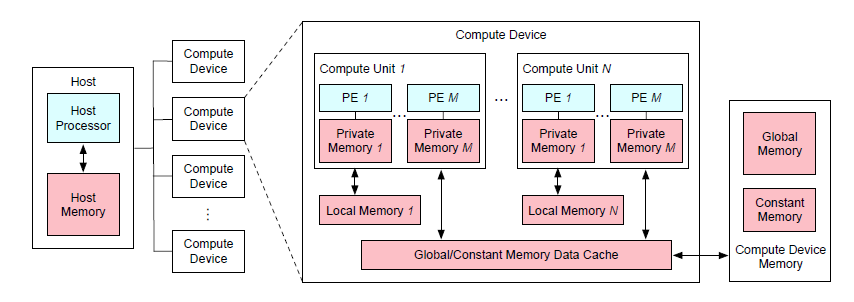
\includegraphics[width=1\textwidth]{OpenCL}
    \caption{The OpenCL platform model and the OpenCL memory model}
    \label{fig:opcl}
  \end{center}
\end{figure}



\section{Overview}

As mentioned before, the previously presented software tools, for both cases (using computers' heterogeneous components and using code parallelization) have their base support even being a programming language, for OpenCL, or a set of compile directives, for OpenMP. Those software tools have improved applications performance somehow, which is already good. However, looking as a software that can do everything on its own, with the minimum programmer's input, in other words, that can do things almost automatically, none of them can make it. The only software tool that is close to that automation is Kremlin because it gives what a developer should do in their code in order to increase its efficiency and performance.

Both approaches, using computers' heterogeneous components and using code parallelization, have the role to answer the state of the art premise: "achieving the highest processing power".  
